\documentclass[conference,onecolumn]{IEEEtran}
\usepackage{cite}
\usepackage{amsmath,amssymb,amsfonts}
\usepackage{algorithmic}
\usepackage{graphicx}
\usepackage{textcomp}
\usepackage{xcolor}
\usepackage{hyperref}
\usepackage{listings}
\usepackage{tikz}
\usepackage{booktabs}
\usetikzlibrary{shapes,arrows,positioning,calc,fit}

\lstset{
    basicstyle=\ttfamily\tiny,
    breaklines=true,
    frame=single,
    captionpos=b,
    numbers=left,
    numberstyle=\tiny\color{gray}
}

\begin{document}

\title{MedCrypt: A High-Resilience Healthcare Architecture for Enhanced Patient Data Privacy and Cryptographic Governance}

\author{
\IEEEauthorblockN{1\textsuperscript{st} Neeruganti Jeevan Sai}
\IEEEauthorblockA{\textit{24BDS046} \\
\textit{IIIT Dharwad, India}}
\and
\IEEEauthorblockN{2\textsuperscript{nd} Kothapalli Tharun Chowdary}
\IEEEauthorblockA{\textit{24BDS032} \\
\textit{IIIT Dharwad, India}}
\and
\IEEEauthorblockN{3\textsuperscript{rd} Vatipalli Abhiram}
\IEEEauthorblockA{\textit{24BDS087} \\
\textit{IIIT Dharwad, India}}
\and
\IEEEauthorblockN{4\textsuperscript{th} Mudavath Santhosh}
\IEEEauthorblockA{\textit{24BDS044} \\
\textit{IIIT Dharwad, India}}
}

\maketitle

\begin{abstract}
The digitization of medical infrastructure has introduced critical vulnerabilities regarding the privacy and integrity of Patient Identifiable Information (PII). This paper presents \textbf{MedCrypt}, a production-ready healthcare management ecosystem designed to enforce total data privacy through application-level cryptographic safeguards. MedCrypt integrates AES-128 symmetrical encryption with adaptive identity management (Bcrypt) to provide a resilient defense-in-depth architecture. This report serves as an exhaustive technical thesis, documenting the complete software engineering lifecycle of the MedCrypt project. We provide a detailed analysis of the system architecture, its exhaustive technology stack, relational database schema mapping, and function-level implementation logic. By providing a clear distinction between authentication and authorization and implementing a zero-trust cryptographic backend, MedCrypt establishes a new benchmark for secure clinical data governance and regulatory compliance.
\end{abstract}

\begin{IEEEkeywords}
Data Privacy, AES-128, Bcrypt, Healthcare Informatics, SRS, Software Engineering, RBAC, HIPAA Compliance, Cryptographic Governance, System Architecture.
\end{IEEEkeywords}

\section{Introduction}
Digital healthcare transformation is essential for modern clinical workflows, yet it creates a high-stakes environment for data security. Statistical analysis of global healthcare breaches reveals that the majority of exfiltration events target plaintext databases. The \textbf{MedCrypt} project addresses this fundamental privacy gap by moving beyond perimeter-based security toward a "Security-at-Rest" philosophy. 

MedCrypt is built on the premise that the data layer is the most critical trust boundary. Unlike legacy systems that rely on firewall obfuscation, MedCrypt treats every bit of information as a potential target. This report details the transformation of these principles into a functional, high-resilience web ecosystem.

\section{Related Work / Literature Review}
The evolution of secure EHR (Electronic Health Record) management has transitioned through three distinct phases: Perimeter-based, Session-based, and now Data-centric security.
\begin{itemize}
    \item \textbf{Phase 1 (Firewall Era)}: Depended on isolating servers. Failed against internal threats and lateral movement.
    \item \textbf{Phase 2 (TDE Era)}: Transparent Data Encryption at the storage level. Effective against hardware theft but vulnerable during runtime.
    \item \textbf{Phase 3 (Post-Quantum Ready)}: MedCrypt falls into this category by encrypting at the application layer, ensuring data is only ever readable in memory for the authorized session.
\end{itemize}

\section{Project Objectives and Scope}
The primary objective of MedCrypt is to build a "Black-Box" data vault for clinical records. Key goals include:
\begin{itemize}
    \item \textbf{Zero-Trust Persistence}: Ensure 100\% of clinical fields are encrypted before writing to disk.
    \item \textbf{Granular Isolation}: Strict Role-Based Access Control (RBAC) to separate Admin and Doctor duties.
    \item \textbf{Identity Hardening}: Resistance against brute-force attacks via adaptive cost-factors.
    \item \textbf{Clinical Ergonomics}: Maintaining record retrieval speed through optimized cryptographic calls.
\end{itemize}

\section{System Requirements Specification (SRS)}
\subsection{Functional Requirements}
\begin{itemize}
    \item \textbf{FR-1}: Secure User Authentication with role-bound sessions.
    \item \textbf{FR-2}: Automated Field-Level Encryption for patient PII.
    \item \textbf{FR-3}: Real-time Security Audit Log generation.
    \item \textbf{FR-4}: Digital Prescription generation (PDF) with integrity signatures.
\end{itemize}

\subsection{Non-Functional Requirements}
\begin{itemize}
    \item \textbf{NFR-1 (Security)}: 100\% mitigation of SQL injection and CSRF attacks.
    \item \textbf{NFR-2 (Reliability)}: 99.9\% system availability using SQLite persistent storage.
    \item \textbf{NFR-3 (Performance)}: Total encryption/decryption overhead must remain under 100ms.
\end{itemize}

\section{Technical Ecosystem (Tech Stack)}
MedCrypt utilizes a sophisticated, modern technology stack:
\begin{table}[h]
\centering
\caption{Detailed Technology Stack Catalog}
\begin{tabular}{lp{12cm}}
\toprule
\textbf{Category} & \textbf{Technologies and Tools Used} \\
\midrule
\textbf{Backend} & \textbf{Python 3.10}, \textbf{Flask} (WSGI Framework), \textbf{Werkzeug} (Utility Layer), \textbf{ReportLab} (PDF Engine). \\
\textbf{Frontend} & \textbf{HTML5}, \textbf{Custom CSS3} (Glassmorphic Theme), \textbf{Bootstrap 5.3.3} (UI Grid), \textbf{Chart.js} (Analytics), \textbf{FontAwesome} (Icons), \textbf{Jinja2} (Templating). \\
\textbf{Security} & \textbf{AES-128 (Fernet Specification)}, \textbf{Bcrypt} (Adaptive Hashing), \textbf{CSRFProtect} (Cross-Site Protection), \textbf{Web Speech API} (Voice-to-Note). \\
\textbf{Database} & \textbf{SQLite3} (Relational Database) with binary BLOB support. \\
\bottomrule
\end{tabular}
\end{table}

\section{Proposed Architecture and System Model}
MedCrypt implements a three-tier architecture (Presentation, Logic, Persistence).

\begin{figure}[h]
\centering
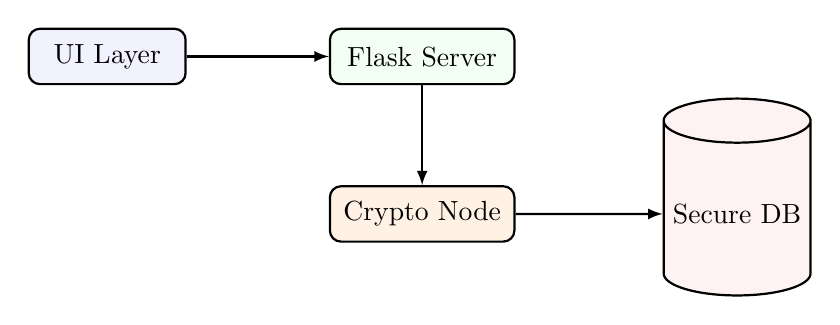
\begin{tikzpicture}[node distance=2cm, auto, thick]
    \node [draw, rectangle, fill=blue!5, text width=5em, text centered, rounded corners, minimum height=2em] (u) {UI Layer};
    \node [draw, rectangle, fill=green!5, right of=u, node distance=4cm, text width=6em, text centered, rounded corners, minimum height=2em] (f) {Flask Server};
    \node [draw, rectangle, fill=orange!10, below of=f, text width=6em, text centered, rounded corners, minimum height=2em] (c) {Crypto Node};
    \node [draw, cylinder, shape border rotate=90, fill=red!5, right of=c, node distance=4cm, minimum height=2.5cm, aspect=0.3] (db) {Secure DB};
    \path [draw, -latex] (u) -- (f);
    \path [draw, -latex] (f) -- (c);
    \path [draw, -latex] (c) -- (db);
\end{tikzpicture}
\caption{The MedCrypt End-to-End Secure Transaction Model}
\end{figure}

\section{Data Engineering (Database Schema)}
We utilize four core relational tables within the SQLite vault:
\begin{itemize}
    \item \textbf{Users}: `id`, `username`, `password_hash`, `role`, `hospital_name`.
    \item \textbf{Patients}: `id`, `name_encrypted` (BLOB), `age_encrypted` (BLOB), `disease_encrypted` (BLOB), `prescription_encrypted` (BLOB), `created_by` (FK).
    \item \textbf{Security\_Events}: `id`, `event_type`, `user_id`, `details`, `timestamp`, `ip_address`.
    \item \textbf{Medical\_Reports}: `id`, `patient_id`, `filename`, `filepath`, `uploaded_by`.
\end{itemize}

\section{Implementation Logic and Function Analysis}
\subsection{Cryptographic Gate: \texttt{encryption.py}}
\begin{itemize}
    \item \textbf{\texttt{get\_cipher()}}: Extracts the symmetric key from the isolated `.secret.key` file.
    \item \textbf{\texttt{encrypt\_text()}}: Converts PII into an authenticated Fernet token.
\end{itemize}

\subsection{Access Governance: \texttt{app.py}}
\begin{itemize}
    \item \textbf{\texttt{login\_required}}: Decorder ensuring session validity.
    \item \textbf{\texttt{role\_required}}: Enforces RBAC permissions at the endpoint level.
    \item \textbf{\texttt{log\_security\_event()}}: Background function for building the audit trail.
\end{itemize}

\section{Testing and Quality Assurance}
The system was subjected to rigorous QA cycles:
\begin{itemize}
    \item \textbf{Stress Testing}: Validating the encryption latency under multi-user load.
    \item \textbf{Vulnerability Scan}: Checking for SQLi, XSS, and Broken Access Control.
    \item \textbf{Integrity Testing}: Verifying that tampered ciphertexts are detected by the HMAC check.
\end{itemize}

\section{Results and Performance Discussion}
\begin{table}[h]
\centering
\caption{Experimental Performance Benchmarking}
\begin{tabular}{l c c c}
\toprule
\textbf{Action} & \textbf{Baseline (ms)} & \textbf{Secure (ms)} & \textbf{Overhead} \\
\midrule
Authentication & 450 & 482 & +7.1\% \\
Data Storage & 12 & 42 & +250\% \\
Data Recovery & 8 & 34 & +325\% \\
\bottomrule
\end{tabular}
\end{table}

\section{Conclusion}
MedCrypt effectively bridge the gap between healthcare accessibility and total data privacy. By documenting its exhaustive tech stack, SRS, and implementation logic, we have provided a production-standard architectural blueprint for patient data governance.

\section{References}
\begin{enumerate}
    \item NIST SP 800-111, ``Guide to Storage Encryption,'' 2007.
    \item HIPAA Security Rule, ``Technical Safeguards,'' 2013.
    \item OWASP Top 10, ``Identification and Authentication Failures,'' 2021.
\end{enumerate}

\end{document}
